\section{Konfiguration der S7-1500} \label{sec: Konfiguration_der_S7_1500}

\subsection{S7-1500 hinzufügen}
Über \glqq\textbf{Neues Gerät hinzufügen}\grqq\:nach \textbf{6ES7 5XX-XXXXX-XXXX} suchen und mit \glqq\textbf{OK}\grqq\:bestätigen.\\
Pfad: Controller > SIMATIC S7-1500 > CPU > Nicht spezifizierte CPU 1500
\begin{figure}[H]
    \centering
   \begin{minipage}[b]{.4\linewidth}
        \centering
        \fbox{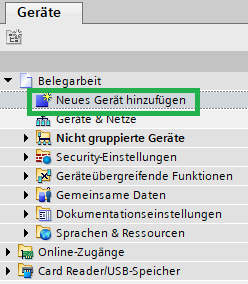
\includegraphics[width=1\linewidth]{Bilder/3. Konfiguration der S7-1500/3.1 S7-1500 hinzufügen/(4) Neues Geraet hinzufuegen.png}}
        \caption[Neues Gerät hinzufügen]{Neues Gerät hinzufügen}
        \label{fig:Bild3.1}
   \end{minipage}
   \hspace{.1\linewidth}% Abstand zwischen Bilder
   \begin{minipage}[b]{.4\linewidth}
        \centering
        \fbox{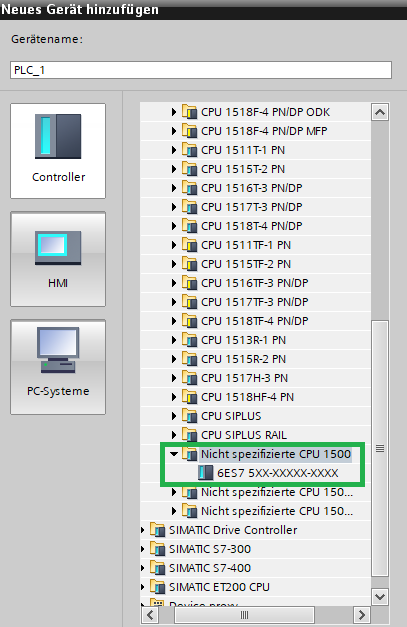
\includegraphics[width=1\linewidth]{Bilder/3. Konfiguration der S7-1500/3.1 S7-1500 hinzufügen/(5) SPS auswaehlen.png}}
        \caption[S7-1500 auswählen]{S7-1500 auswählen}
        \label{fig:Bild3.2}
   \end{minipage}
\end{figure}

\clearpage

\subsection{Kommunikation herstellen}
In der \textbf{Gerätesicht} der S7-1500 über \glqq\textbf{ermitteln}\grqq\:die entsprechende Hardware suchen.
\begin{figure}[H]
   \centering
   \fbox{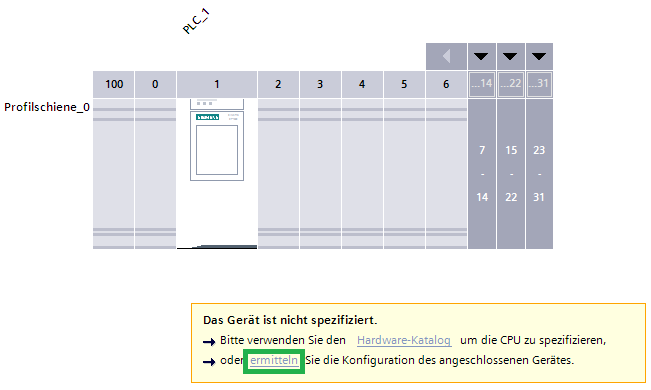
\includegraphics[width=0.7\textwidth]{Bilder/3. Konfiguration der S7-1500/3.2 Kommunikation herstellen/(6) Hardware ermitteln.png}}
   \caption[Hardware ermitteln]{Hardware ermitteln}
   \label{fig:Bild3.3}
\end{figure}

Einstellungen der Schnittstelle vornehmen und mit \glqq\textbf{Suche starten}\grqq\:nach Geräten suchen. Anschließend das richtige Gerät anhand der IP-Adresse (hier: 192.168.1.116) auswählen und mit \glqq\textbf{Erkennen}\grqq\:bestätigen.
\begin{figure}[H]
   \centering
   \fbox{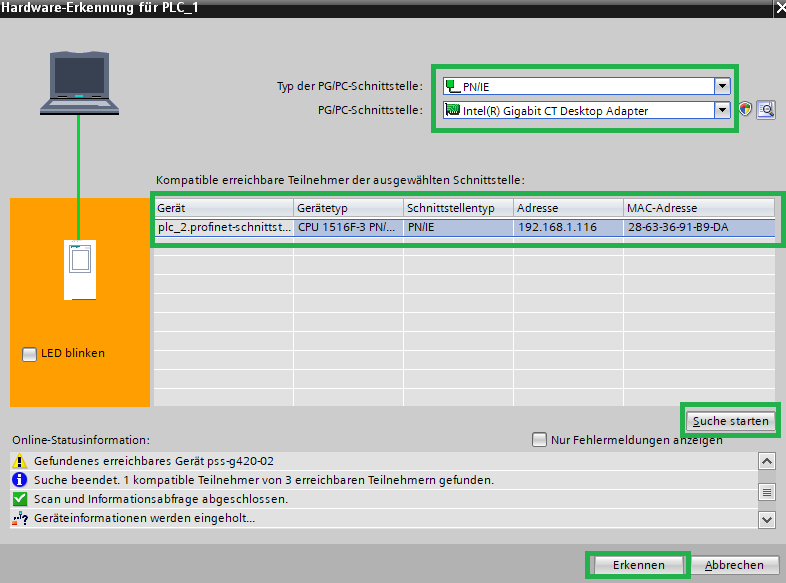
\includegraphics[width=0.6\textwidth]{Bilder/3. Konfiguration der S7-1500/3.2 Kommunikation herstellen/(7) Kommunikation aufnehmen.png}}
   \caption[Kommunikation herstellen]{Kommunikation herstellen}
   \label{fig:Bild3.4}
\end{figure}

\subsection{Security-Einstellungen der S7-1500}
Nachdem das Gerät erkannt wurde, öffnet sich das Fenster \textbf{PLC Security-Einstellungen}.\\
\newline
1. Schutz vertraulicher PLC-Konfigurationsdaten \textbf{deaktivieren}:
\begin{figure}[H]
   \centering
   \fbox{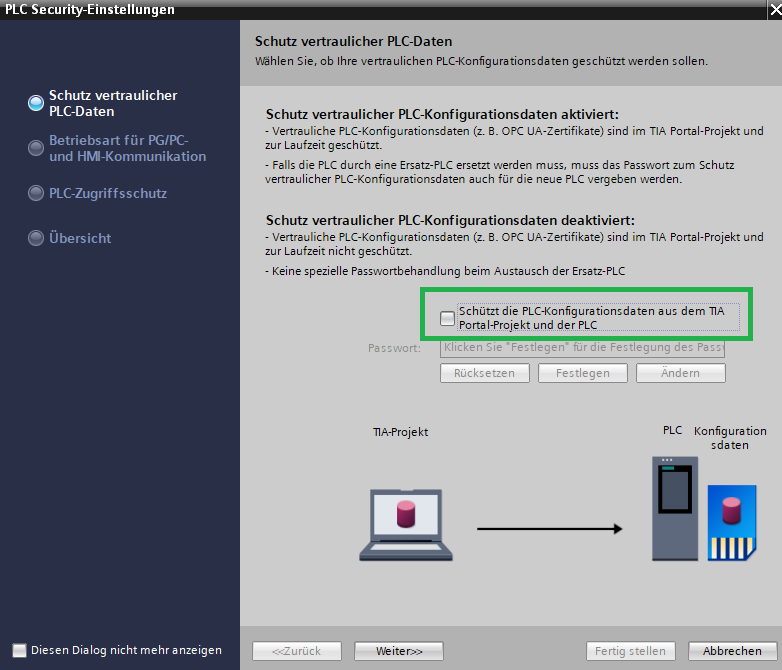
\includegraphics[width=0.8\textwidth]{Bilder/3. Konfiguration der S7-1500/3.3 Security-Einstellungen der S7-1500/(7.1) Security Einstellungen (1).png}}
   \caption[Security Einstellungen Teil 1]{Security Einstellungen Teil 1}
   \label{fig:Bild3.5}
\end{figure}

\clearpage

2. Legacy- und Secure PG/PC-Kommunikation \textbf{nicht zulassen}:
\begin{figure}[H]
   \centering
   \fbox{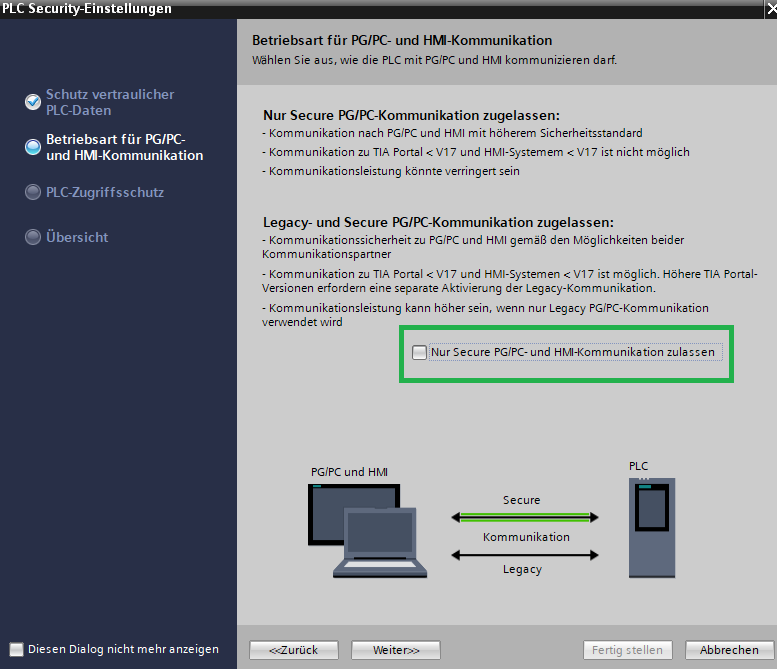
\includegraphics[width=0.8\textwidth]{Bilder/3. Konfiguration der S7-1500/3.3 Security-Einstellungen der S7-1500/(7.2) Security Einstellungen (2).png}}
   \caption[Security Einstellungen Teil 2]{Security Einstellungen Teil 2}
   \label{fig:Bild3.6}
\end{figure}

\clearpage

3. Zugriffstufe ohne Passwort auf \textbf{Vollzugriff inkl. fehlersicher (kein Schutz)} stellen:
\begin{figure}[H]
   \centering
   \fbox{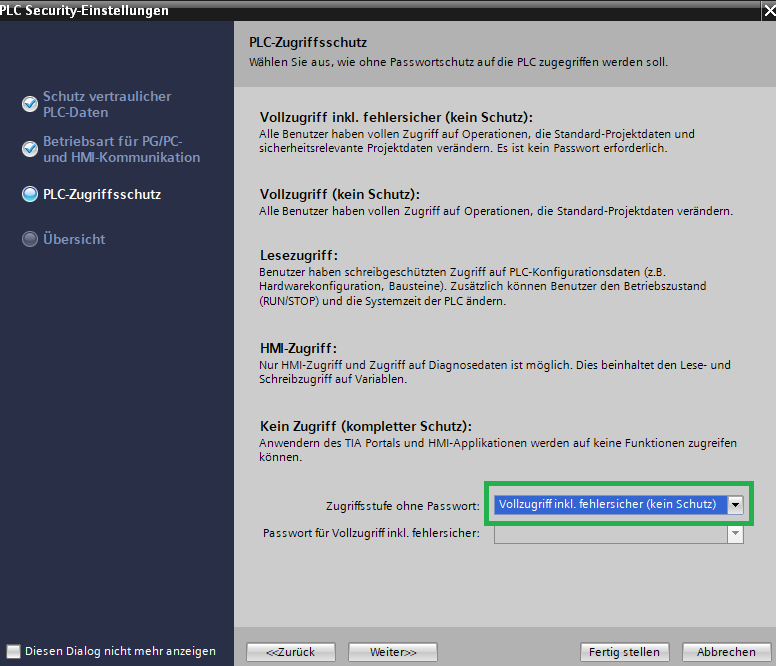
\includegraphics[width=0.8\textwidth]{Bilder/3. Konfiguration der S7-1500/3.3 Security-Einstellungen der S7-1500/(7.3) Security Einstellungen (3).png}}
   \caption[Security Einstellungen Teil 3]{Security Einstellungen Teil 3}
   \label{fig:Bild3.7}
\end{figure}

Die Einstellungen mit \glqq\textbf{Fertig stellen}\grqq\:übernehmen. Zuletzt über die \textbf{Gerätesicht} der S7-1500 den \textbf{Schreibzugriff deaktivieren}.\\
Pfad: Allgemein > Display > Passwort 
\begin{figure}[H]
   \centering
   \fbox{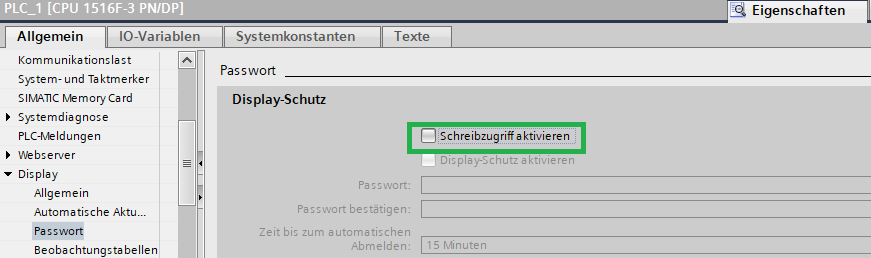
\includegraphics[width=0.8\textwidth]{Bilder/3. Konfiguration der S7-1500/3.3 Security-Einstellungen der S7-1500/(8) Passwortschutz entfernen.png}}
   \caption[Passwortschutz entfernen]{Passwortschutz entfernen}
   \label{fig:Bild3.8}
\end{figure}

\clearpage

\subsection{IP-Adresse und Vergabe des PROFINET-Gerätenamen der S7-1500} \label{sec: IP-Adresse_PROFINET-Gerätename_S7-1500}
Die jeweiligen IP-Adressen und PROFINET-Gerätenamen können der \autoref{fig:Bild1.3} entnommen werden. Die Bezeichnung des PROFINET-Anschlusses ist \textbf{X2}.

\begin{figure}[H]
   \centering
   \fbox{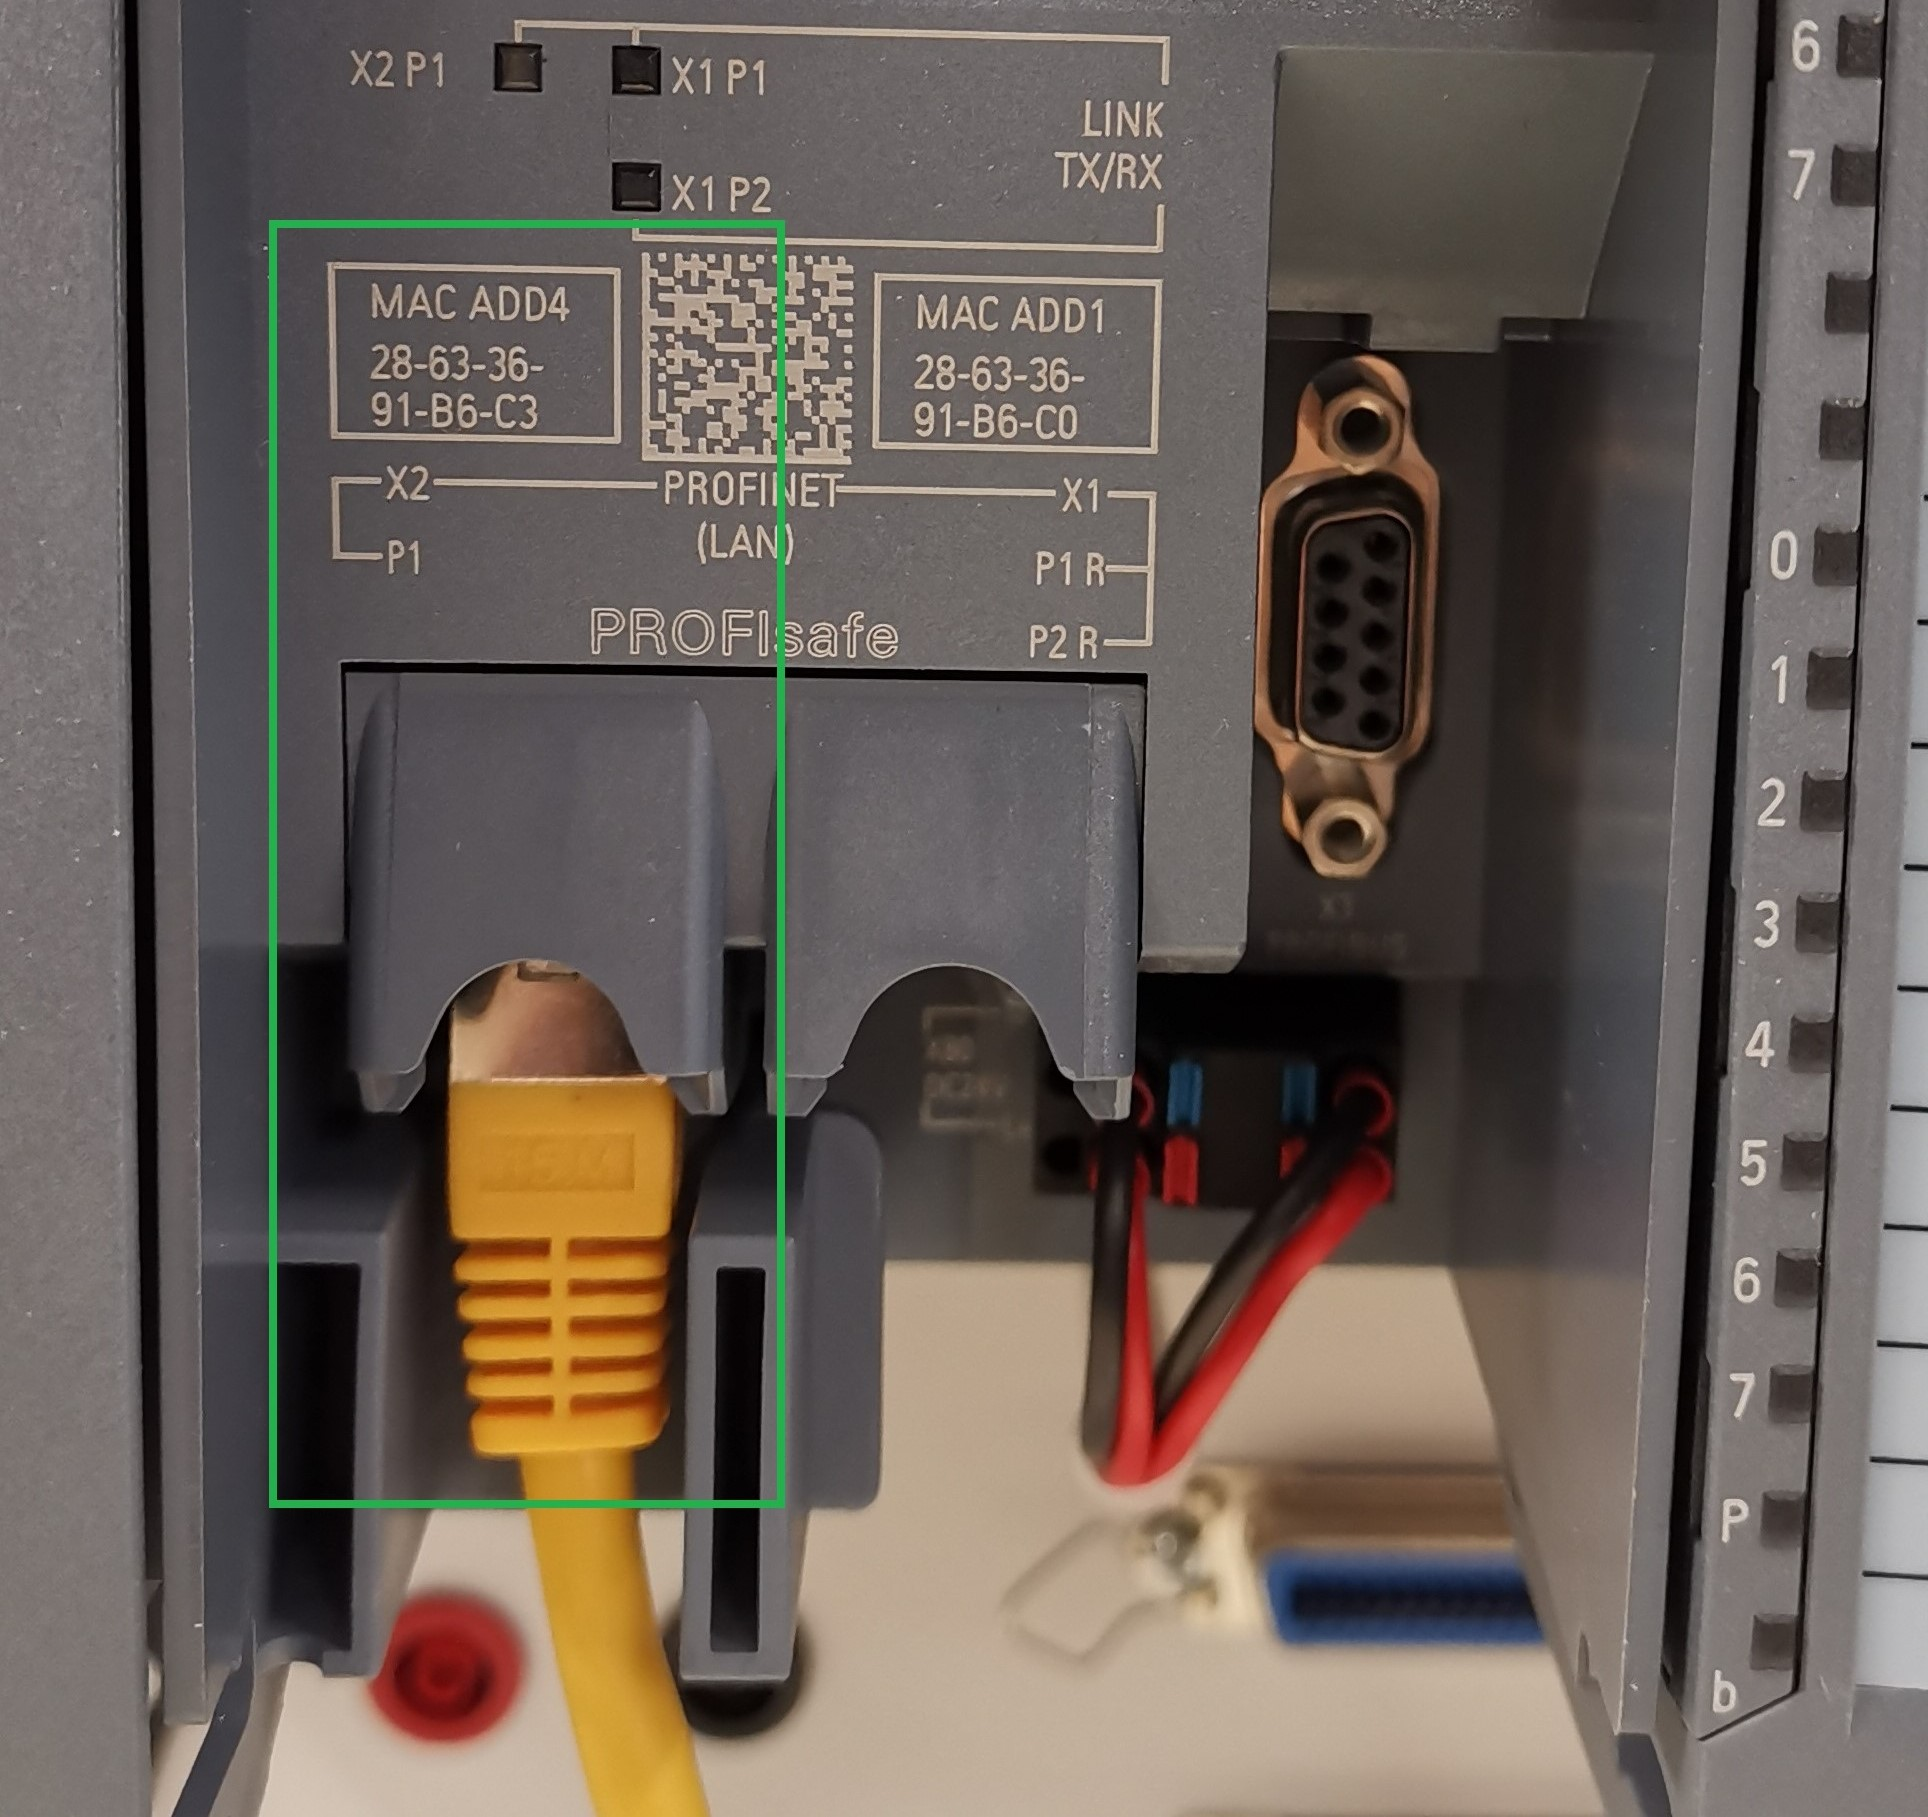
\includegraphics[width=0.45\textwidth]{Bilder/3. Konfiguration der S7-1500/3.4 IP-Adresse und Vergabe des PROFINET-Gerätenamen der S7-1500/(9.1) PROFINET-Schnittstelle.jpg}}
   \caption[Anschluss an PROFINET-Schnittstelle]{Anschluss an PROFINET-Schnittstelle}
   \label{fig:Bild3.9}
\end{figure}

1. IP-Adresse vergeben:\\
Pfad über \textbf{Gerätesicht}: Allgemein > PROFINET-Schnittstelle [X2] > Ethernet-Adressen
\begin{figure}[H]
   \centering
   \fbox{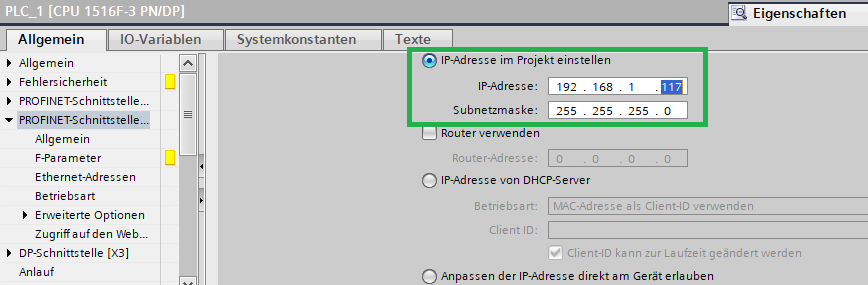
\includegraphics[width=0.9\textwidth]{Bilder/3. Konfiguration der S7-1500/3.4 IP-Adresse und Vergabe des PROFINET-Gerätenamen der S7-1500/(9.2) IP-Adresse der S7 einstellen.png}}
   \caption[IP-Adresse der S7-1500 eingeben]{IP-Adresse der S7-1500 eingeben}
   \label{fig:Bild3.10}
\end{figure}

Zur Eingabe des PROFINET-Gerätenamen das Häkchen bei \glqq\textbf{PROFINET-Gerätename automatisch generieren}\grqq\:entfernen.\\
2. PROFINET-Gerätename vergeben:\\
Pfad über \textbf{Gerätesicht}: Allgemein > PROFINET-Schnittstelle [X2] > Ethernet-Adressen
\begin{figure}[H]
   \centering
   \fbox{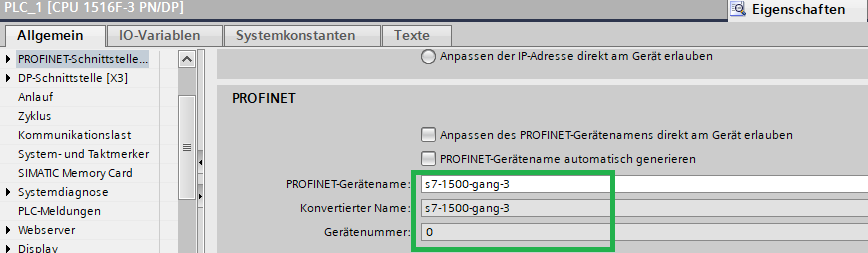
\includegraphics[width=0.9\textwidth]{Bilder/3. Konfiguration der S7-1500/3.4 IP-Adresse und Vergabe des PROFINET-Gerätenamen der S7-1500/(9.3) PROFINET-Geraetename S7 einstellen.png}}
   \caption[PROFINET-Gerätename der S7-1500 eingeben]{PROFINET-Gerätename der S7-1500 eingeben}
   \label{fig:Bild3.11}
\end{figure}